\documentclass{article}
\usepackage{tikz}
\begin{document}
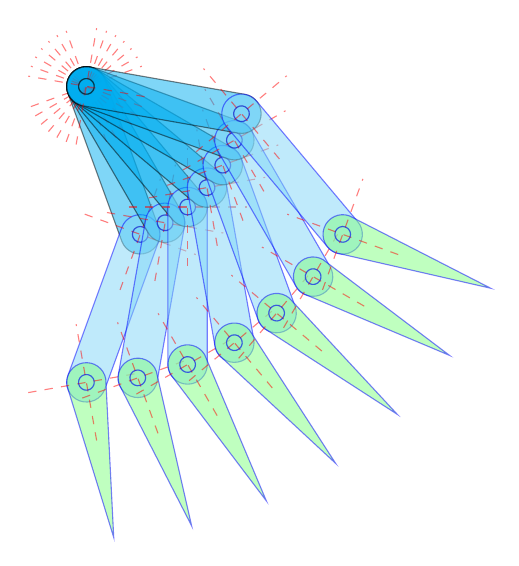
\begin{tikzpicture}
\foreach \a in {20,30,...,80}{
\begin{scope}[rotate=\a,opacity=.5]
	\coordinate (P1) at (0,0);
	\draw[fill=cyan] (P1)++(-.25,0) -- ++(0,-2) arc (180:360:.25) -- ++(0,2) arc (0:180:.25);
	\draw[red,dashed] (P1)++(-.75,0) -- ++(1.5,0) (P1)++(0,-.75) -- ++(0,1.5);
	\draw (P1) circle (.1);
	\draw (P1)++(0,-2) circle (.1);
	\begin{scope}[shift={(0,-2)},rotate=-40,blue]
		\coordinate (P2) at (0,0);
		\draw[fill=cyan!50] (P2)++(-.25,0) -- ++(0,-2) arc (180:360:.25) -- ++(0,2) arc (0:180:.25);
	\draw[red,dashed] (P2)++(-.75,0) -- ++(1.5,0) (P2)++(0,-.75) -- ++(0,1.5);
	\draw (P2) circle (.1);
	\draw (P2)++(0,-2) circle (.1);
		\begin{scope}[shift={(0,-2)},rotate=30,blue]
			\coordinate (P3) at (0,0);
			\draw[fill=green!50] (P3)++(-.25,0) -- ++(.25,-2) -- ++(.25,2) arc (0:180:.25);
			\draw[red,dashed] (P3)++(-.75,0) -- ++(1.5,0) 	(P3)++(0,-.75) -- ++(0,1.5);
			\draw (P3) circle (.1);
		\end{scope}
	\end{scope}
\end{scope}
}
\end{tikzpicture}
\end{document}
